\documentclass{article}
\usepackage{booktabs} % For better-looking tables
\usepackage{graphicx}
\begin{document}
\begin{figure}[ht]
    \centering
    
\includegraphics[width=0.5\textwidth]{images/HairCut.png}
    \caption{HairCut application Icon}
    \label{fig: exmaple}
\end{figure}
\begin{table}[h] % Place the table "here" (h) on the page
    \centering
    \begin{tabular}{|c |c|} \hline  % Define the number of columns and their alignment
        
        Names& ID\\ \hline 
        
        Marwan Almehmadi& 1741630
\\ \hline 
        Anas Aldhahri& 1845490\\ \hline 
        
 Waleed Aldhahri&2042395\\ \hline 
 Abdulrahman Maghrabi&2042791\\ \hline 
 Ali Abualwah&2140185\\ \hline 
 Sari Alblwi&2142407\\ \hline 
 Supervisor&Sakher Ghanem\\ \hline
    \end{tabular}
    \caption{Names and IDs}
    \label{tab:yourtablelabel}
\end{table}
\newpage
{Chapter 5: Implementation}
\begin{itemize}
\item \subsection{Report Outline:}
\begin{itemize}

\item \textbf{Introduction:} An Introduction to the chapter.

\item \textbf{Software Description:} Details of the used libraries , frameworks and IDE(s) in addition to design tools along with the used programming languages.

\item \textbf{Hardware Description:} The required operating system of the mobile phone used in this project along the specification and version of the operating system.

\item \textbf{Details:} Description of the frontend and user interface.

\item \textbf{Conclusion:} Conclusion of the chapter. 
\end{itemize}

\item \subsection{Introduction:}

In this chapter, we are going to discuss and describe software tools and IDEs that we are going to use in the project, hardware components needed for the project to function and work properly, and finally the details surrounding the implementation process, and how we implement the hardware and software elements together so the project functions as intended.
\newpage
\item \subsection{Software Description}
\begin{figure}[ht]
    \centering
    
\includegraphics[width=0.5\textwidth]{images/Android studio.png}
    \caption{Android Studio Icon}
    \label{fig: }
\end{figure}
In this section, we are going to describe the software tools and IDEs that we are going to use in this project, starting with Android studio, it is an IDE used for the development of mobile applications, It is based on JetBrains' IntelliJ IDEA software and tailored specifically for Android development. Android Studio offers a comprehensive set of tools for designing, building, and testing Android applications. 
\newpage
\begin{figure}[ht]
    \centering
    
\includegraphics[width=0.5\textwidth]{images/Kotlin_Icon.png}
    \caption{Kotlin Icon}
    \label{fig: exmaple}
\end{figure}

As for the programming language, we are going to use Kotlin, it is a programming language that runs on the Java Virtual Machine (JVM) and also compiles to JavaScript or native code. Developed by JetBrains, the creators of popular IDEs like IntelliJ IDEA Here are some key points about Kotlin:

\textbf{Conciseness and Readability:} Kotlin is designed to be concise, reducing the amount of boilerplate code compared to Java.

 \textbf{Interoperability:} Kotlin is fully interoperable with Java, allowing developers to use Kotlin and Java code together within the same project. 
 
\textbf{Null Safety:} Kotlin addresses the common issue of null pointer exceptions by making null safety a core feature of the language.
 
Overall, Kotlin has gained popularity among developers for its modern features, seamless interoperability with existing Java codebases, and its focus on safety, conciseness, and expressiveness.

\newpage

\begin{figure}[h]
    \centering
    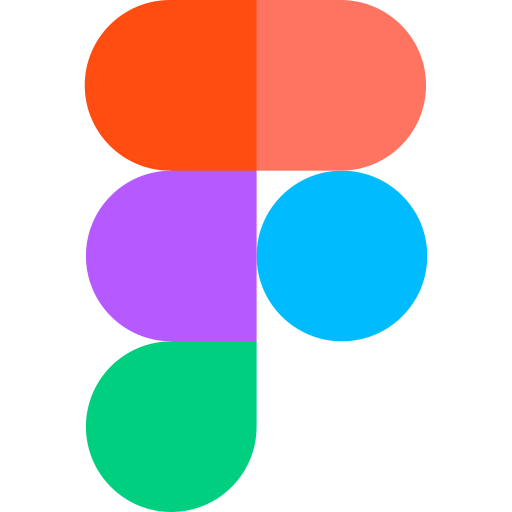
\includegraphics[width=0.5\textwidth]{images/Figma.png}
    \caption{Figma Icon}
    \label{fig: exmaple}
\end{figure}

As for the \textbf{front end} design, we used the\textbf{\textit{ }figma} program/website to design the front end, including the User interfaces and such, figma is a cloud-based design tool used for interface design, prototyping, and collaboration. It was developed by Figma, Inc. Here are some key aspects of Figma:

\textbf{Cloud-Based Design Tool:} Figma is a web-based tool that allows designers to create, prototype, and collaborate on designs in real-time.

 
\textbf{Vector Graphics Editor:} Figma is equipped with powerful vector editing tools that enable designers to create and manipulate scalable vector graphics (SVG) for designing user interfaces, icons, illustrations, and more.

 \textbf{Prototyping and Interaction Design:} Designers can create interactive prototypes in Figma by linking different frames and designing transitions, animations, and interactions.  
 Figma has become a go-to tool for many designers and design teams due to its user-friendly interface, collaborative capabilities, and comprehensive set of features that support the end-to-end design process. 
 
\newpage

\item \subsection{Hardware Description}
In this section we are going to describe the hardware components and the requirements and specifications needed for the app to run on the hardware without any issues, we are going to use Android pixel to run the application on, the required storage space would be at least 300 MB, and the RAM (Random Access Memory) needed is at least 4GB RAM for the app to run properly. The Android pixel device is a test device for the application, any other android device that meets the requirements will run the application without any issues.

 \begin{figure}[h]
    \centering
    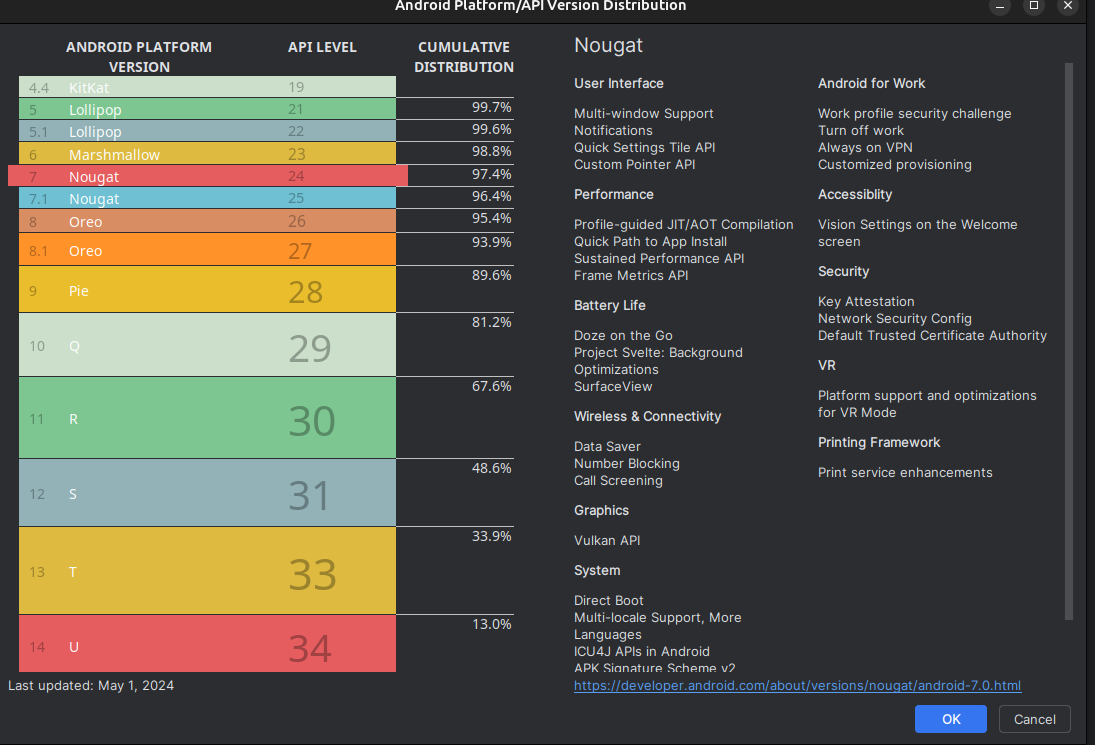
\includegraphics[width=0.5\textwidth]{images/Android platform chart.png}
    \caption{Android platform chart of each platform's distribution}
    \label{fig: exmaple}
\end{figure}
\item \subsection{Details}
In this section of the report we discuss the user interface in steps with description of each page and the present components
in addition to the flow of the pages and the difference between each user. 

\begin{figure}[h]
    \centering
    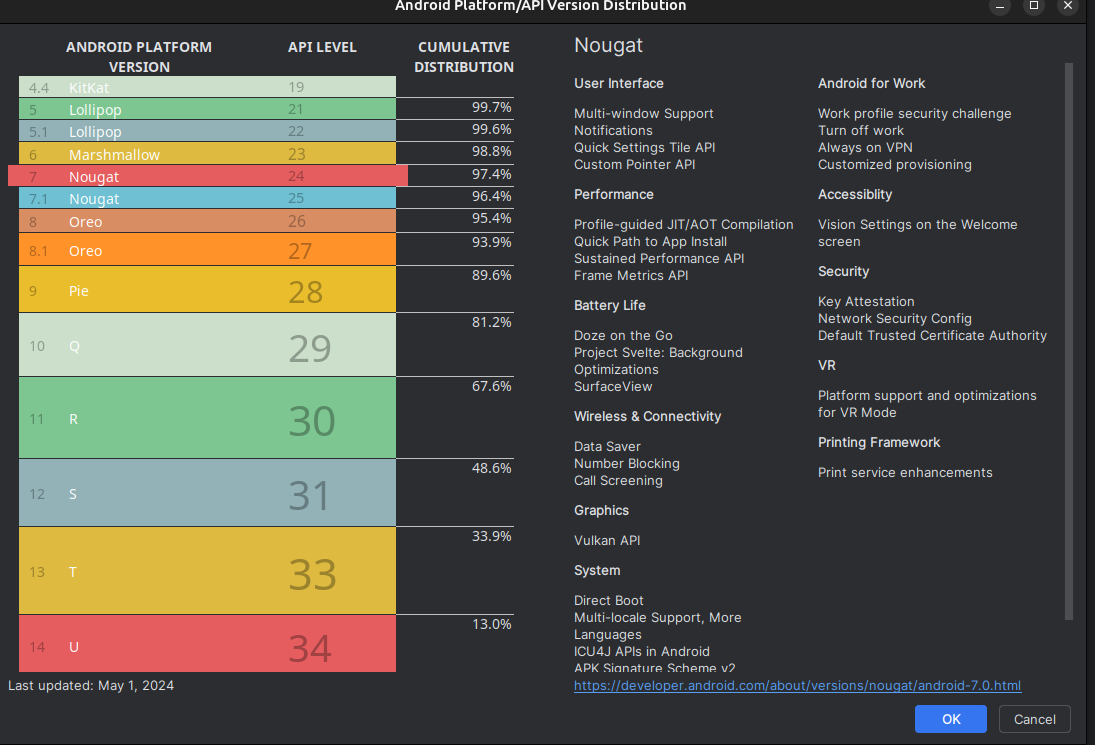
\includegraphics[width=0.5\textwidth]{images/Android platform chart.png}
    \caption{Android platform chart of each platform's distribution}
    \label{fig: exmaple}
\end{figure}
\newpage
Firstly, the application starts by the `welcome page' which displays several options of kind of users the application is going to serve
and the users are categorized as follows:
\begin{figure}[h]
    \centering
    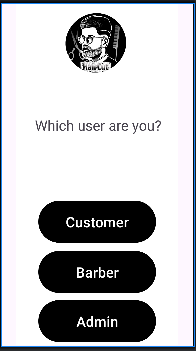
\includegraphics[width=0.5\textwidth]{images/user_classification.png}
    \caption{Android platform chart of each platform's distribution}
    \label{fig: User classification screen}
\end{figure}

\begin{itemize}
    \item Customer
    \item Barber
    \item Admin
\end{itemize}
\newpage

Secondly, after the user clicks on the suitable option another page asks the user whether they are trying to login or signup for the first time.


\begin{figure}[h]
    \centering
    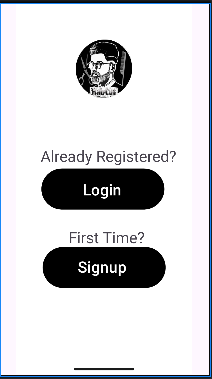
\includegraphics[width=0.5\textwidth]{images/signup_or_login.png}
    \caption{Android platform chart of each platform's distribution}
    \label{fig: User classification screen}
\end{figure}

\begin{figure}[h]
    \centering
    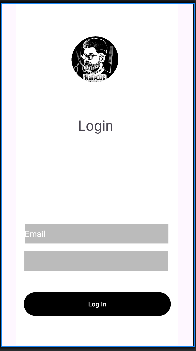
\includegraphics[width=0.5\textwidth]{images/login_page.png}
    \caption{Android platform chart of each platform's distribution}
    \label{fig: User classification screen}
\end{figure}

\item \subsection{Conclusion}

\end{itemize}

\end{document}